\documentclass[a4paper]{article}

\usepackage{fullpage} % Package to use full page
\usepackage{parskip} % Package to tweak paragraph skipping
\usepackage{tikz} % Package for drawing
\usepackage{amsmath}
\usepackage{hyperref}
\usepackage{listings}
\usepackage[framed,numbered,autolinebreaks,useliterate]{mcode}
\title{Numerical Implementation of Fourier Galerkin Method}
\author{Quanhui Zhu}

\begin{document}

\maketitle

\section{Introduction}

The Fourier-Galerkin Method is to solve the differential equations with periodic boundary conditions. We project the solutions from infinite dimensional space into finite dimensional space $\hat{B_N}=span\{e^{inx}|n\le N/2\}$.

The numerical solution $u_h=\sum\limits_{n=-N/2}^{N/2}\hat{u}_ne^{inx_h}$,  where $x_j=\frac{2\pi j}{N}, j=0,1,\cdots,N-1$ are the nodes of the domain
and $\hat{u}_n$ are the Fourier coefficients given by
\begin{equation}
    \hat{u}_n=\frac{1}{2\pi}\int_0^{2\pi}u(x)e^{-inx}dx
    \label{eq::coefficient}
\end{equation}

In discrete cases, it can be rewritten by 
\begin{equation}
    \hat{u}_n=\frac{1}{N}\sum\limits_{j=0}^{N-1}u(x_j)e^{-inx_j}
    \label{eq::hatu}
\end{equation}

For the differential equations 
\begin{equation}
    u_t=\mathcal{L}u+\mathcal{N}u
    \label{problem}
\end{equation} 
the numerical problem using semi-implicit scheme can be rewritten by 
\begin{equation}
    \frac{u^{n+1}-u^n}{\delta t}=\mathcal{L}u^{n+1}+\mathcal{N}u^n.
\end{equation}
Then we calculate the problem in spectral space
\begin{equation}
     \frac{\hat{u}_k^{n+1}-\hat{u}_k^n}{\delta t}=f(k)\hat{u}_k^{n+1}+\hat{(\mathcal{N}u^n)}_k.
     \label{eq::time_scheme}
\end{equation}
The matrix is diagonal.

\section{Matching with Matlab FFT}
\subsection{1-D Match}
Assume the number of the nodes is $2N+1$(odd), the even nodes have a little difference.

In matlab the ifft function is
\begin{equation}
    X(k)=\frac{1}{2N+1}\sum_{j=1}^{2N+1}x(j)e^{\frac{2\pi i(j-1)(k-1)}{2N+1}},\quad k = 1:2N+1.
\end{equation}
For matching
\begin{equation}
    \hat{u}_n=\frac{1}{2N+1}\sum_{j=0}^{2N}u_je^{\frac{2\pi ijn}{2N+1}},\quad n = -N:N,
\end{equation}
we shift $k=n+N+1$, thus 
\begin{equation}
    \hat{u}_n=\frac{1}{2N+1}\sum_{j=1}^{2N+1}u_{j-1}e^{\frac{2\pi i(j-1)(k-N-1)}{2N+1}}
    =\frac{1}{2N+1}\sum_{j=1}^{2N+1}u_{j-1}e^{\frac{-2N\pi i(j-1)}{2N+1}}e^{\frac{2\pi i(j-1)(k-1)}{2N+1}}
\end{equation}

So we can obtain $\hat{u}=ifft(\{u_{j-1}e^{\frac{-2N\pi i(j-1)}{2N+1}}\}_j)$.

Similarly, we can obtain $u=\{e^{\frac{-2N\pi i(j-1)}{2N+1}}\}_j.*fft(\hat{u})$.

\subsection{Arbitrary Period}
When the domain changes $x\in [a,b]$, we have $x_j=\frac{b-a}{2N+1}j+a,\quad j=0,\cdots,2N$. It just need a shift to the domain $[0,2\pi]$,
\begin{equation}
    y=\frac{2\pi}{b-a}(x-a)
\end{equation}
So we have the spectral 
\begin{equation}
    \hat{u}_n=\frac{1}{2N+1}\sum_{j=1}^{2N+1}u_{j-1}e^{in\frac{2\pi}{b-a}(x_{j-1}-a)}=\frac{1}{2N+1}\sum_{j=1}^{2N+1}u_{j-1}e^{\frac{2\pi in(j-1)}{2N+1}}
\end{equation}
Then the transform is the same.

\subsection{2-D Match}
In the domain $[0,2\pi]\times[0,2\pi]$, assume the number of the nodes is $(2N+1)\cdot(2N+1)$.

In matlab the ifft2 is the 2-D Inverse Fast Fourier Transform which has the equation that
\begin{equation}
    Y_{p,q}=\frac{1}{mn}\sum_{j=1}^{m}\sum_{k=1}^{n}X_{j,k}\omega_m^{(j-1)(p-1)}\omega_n^{(k-1)(q-1)}
\end{equation}
where $\omega_N=e^{\frac{2\pi i}{N}}$.

It's the same with 1-D's transform. For matching with the textbook, we just need to shift both in x and y direction. We have 
\begin{equation}
    \hat{u}_{p,q}=\frac{1}{(2N+1)^2}\sum_{j=1}^{2N+1}\sum_{j=1}^{2N+1}u_{j-1,k-1}\cdot e^{\frac{-2N\pi i(j-1)}{2N+1}}\cdot e^{\frac{-2N\pi i(k-1)}{2N+1}}\omega_m^{(j-1)(p-1)}\omega_n^{(k-1)(q-1)}
\end{equation}
Assume 
\begin{equation}
    y_{j,k}=u_{j,k}\cdot e^{\frac{-2N\pi ij}{2N+1}}\cdot e^{\frac{-2N\pi ik}{2N+1}},\quad j=0:2N, k=0:2N
\end{equation}
Thus we have $\hat{u}=ifft2(y)$.

Similarly, assume $z=fft2(\hat{u})$, we have 
\begin{equation}
    u_{j,k}=z_{j,k}\cdot e^{\frac{2N\pi ij}{2N+1}}\cdot e^{\frac{2N\pi ik}{2N+1}}, j=0:2N, k=0:2N
\end{equation}

\section{Numerical Examples}
\subsection{Diffusion Equation}
The equation is 
\begin{equation}
    -u_{xx}=f.
\end{equation}
Using Fourier galerkin method with periodic boundary condition, the equation can rewritten as
\begin{equation}
\begin{array}{cc}
    -\sum\limits_{n=-\frac{N}{2}}^{\frac{N}{2}}\hat{u}_n(e^{inx})_{xx}=\sum\limits_{n=-\frac{N}{2}}^{\frac{N}{2}}\hat{f}_ne^{inx};\\
    i.e.\qquad n^2\hat{u}_n=\hat{f}_n,\qquad n=-\frac{N}{2}:\frac{N}{2}.
    \end{array}
\end{equation}
Notice that when $n=0$, we have $\hat{f}_0=\frac{1}{N}\sum\limits_jf(x_j)=0$ which is called compatibility condition. And the numerical solution is $u_h=\sum\limits_{n=-\frac{N}{2},n\neq0}^{\frac{N}{2}}\hat{u}_ne^{inx}+\hat{u}_0$, where $\hat{u}_0=\frac{1}{N}\sum\limits_j u(x_j)$ called stability condition should be given.

Firstly we calculate $u=sin2x$ to test. $u=sin2x$ shall be exact for any $N$ since it is a base of $B_N$.
When $N=10$, the residual is less than $1e-15$. This test can show whether your codes have grammar error.

Secondly we calculate $u=\frac{3}{5-4cosx}$ and observe how the residual changes with $N$ changing.
\begin{figure}[h]
    \centering
    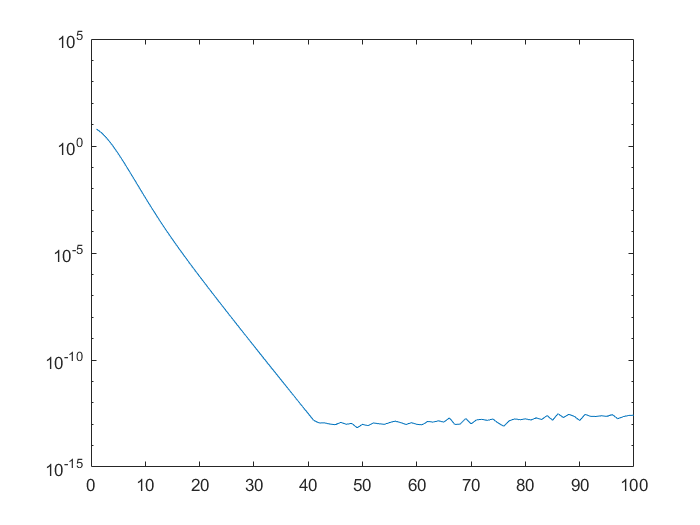
\includegraphics[scale=0.5]{convergence.png}
    \caption{The x-axis is $\frac{N-1}{2}$ where N is the number of nodes and the y-axis is $ln(error)$ where the error is $||u-u_h||_{L^\infty}$.}
    \label{im::convergence}
\end{figure}

In Figure \ref{im::convergence} it follows $||u-u_h||=e^{-N}$ until the error attains machine epsilon.

After these two tests finished, the program is much possible to be right and we shall use the method to solve typical problem now.

\subsection{1-D Allen Cahn Equation}
The equation is
\begin{equation}
    u_t=\epsilon u_{xx}+u-u^3.
\end{equation}
Using Fourier galerkin method and semi-implicit scheme, the iteration takes the form as
\begin{equation}
    \frac{\hat{u}_k^{n+1}-\hat{u}_k^n}{\delta t}=-\epsilon k^2\hat{u}_k^{n+1}+\hat{(u^n-(u^n)^3)}_k,
\end{equation}
where $\delta t$ depends on $\epsilon$ and $h$.

Here is a numerical experiment. Set $\Omega = [0,2\pi], N = 40, \delta=\frac{1}{N^2}, T=1, \epsilon=0.01$ and $u(x,0)=sin(x)$.
Figure \ref{im::1D_Allen_Cahn}  shows the numerical solution.
\begin{figure}[h]
    \centering
    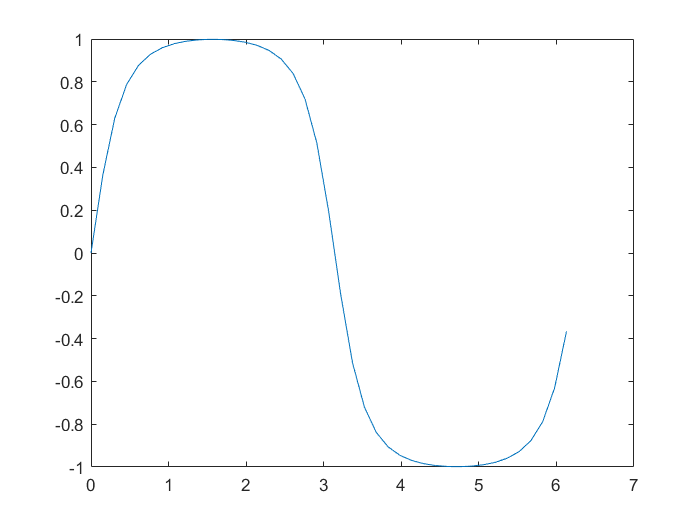
\includegraphics[scale=0.5]{allen_cahn.png}
    \caption{The Allen-Cahn equation's solution when $T=1$ and $\Omega = [0,2\pi], N = 40, \delta t=\frac{1}{N^2}, \epsilon=0.01, u(x,0)=sin(x)$.}
    \label{im::1D_Allen_Cahn}
\end{figure}

\subsection{2-D Allen Cahn Equation}
The equation is the same
\begin{equation}
    u_t = \epsilon \Delta u +u-u^3.
\end{equation}
Using Fourier galerkin method and semi-implicit scheme, similarly the iteration takes the form as 
\begin{equation}
    \frac{\hat{u}_{p,q}^{n+1}-\hat{u}_{p,q}^n}{\delta t}=-\epsilon (p^2+q^2)\hat{u}_{p,q}^{n+1}+\hat{(u^n-(u^n)^3)}_{p,q}.
\end{equation}
Figure \ref{im::2D_Allen_Cahn_sinxsiny} and Figure \ref{im::2D_Allen_Cahn_rand} are two numerical examples.
\begin{figure}[h]
    \centering
    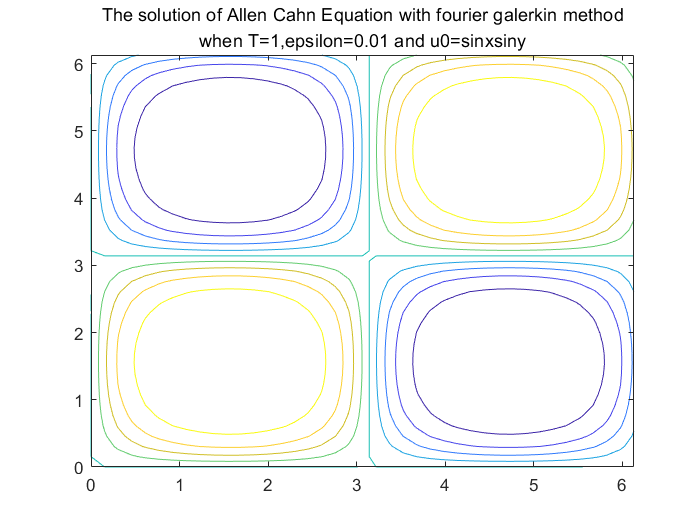
\includegraphics[scale=0.4]{2DAllen_Cahn.png}
    \caption{The 2D Allen-Cahn equation's solution when $T=1$ and $\Omega = [0,2\pi]\times[0,2\pi], N = 20, \delta=0.001, \epsilon=0.01, u(x,0)=sin(x)sin(y)$. It's similar with 1D's.}
    \label{im::2D_Allen_Cahn_sinxsiny}
\end{figure}
\begin{figure}[h]
    \centering
    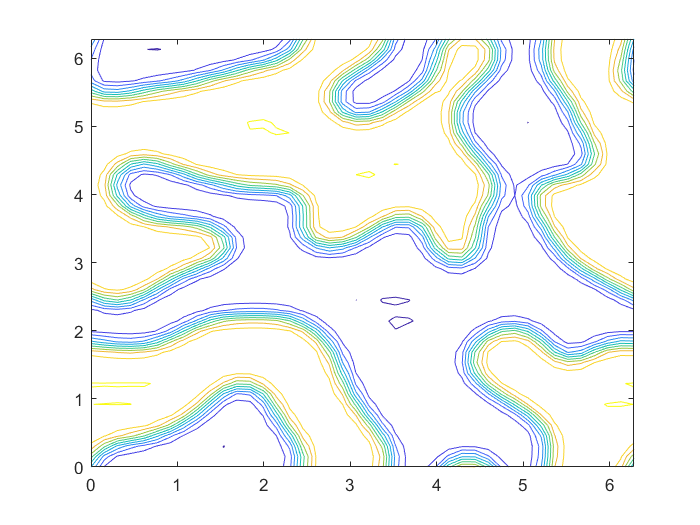
\includegraphics[scale=0.4]{2DAllen_Cahn2.png}
    \caption{The 2D Allen-Cahn equation's solution when $T=10$ and $\Omega = [0,2\pi]\times[0,2\pi], N = 20, \delta t=0.001, \epsilon=0.01, u(x,0)$ are random numbers in [-1,1]. The figure shows most of $u$ get to -1 or 1 and the interface changes quickly.}
    \label{im::2D_Allen_Cahn_rand}
\end{figure}
\newpage
\subsection{Cahn-Hailliard}
Consider the Cahn-Hailliard equation
\begin{equation}
\begin{array}{rccl}
    \frac{\partial u}{\partial t}&=&\Delta(-\epsilon^2\Delta u +f(u)),&\quad x\in\Omega, t\in[0,T],\\
    u(x,0)&=&u_0(x),&\quad x\in \Omega,
\end{array}
\end{equation}
where the $f(u)=u^3-u$.
By Fourier Spectral Transform, the equation can be rewritten with the form of 
\begin{equation}
    \frac{\hat{u}^{n+1}_{p,q}-\hat{u}^{n}_{p,q}}{\delta t}=-\epsilon^2(p^2+q^2)^2\hat{u}^{n+1}_{p,q}+(p^2+q^2)\hat{f(u)}_{p,q}.
\end{equation}
Here are three numerical solutions of Cahn-Hailliard equation.

\begin{figure}[h]
    \centering
    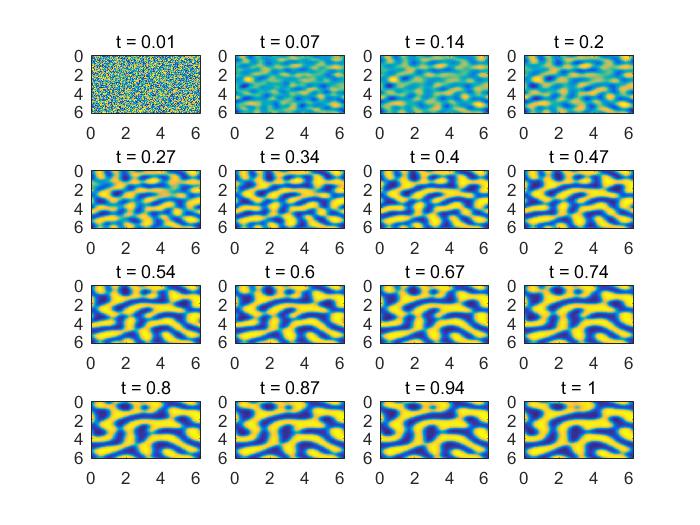
\includegraphics[scale=0.5]{2DCahn_Hilliard_Time[0,1].png}
    \caption{The time procedure of Cahn-Hailliard equation where $dt = 0.001, \epsilon^2=0.01, N=100, u0=rand(-1,1)$}
    \label{im::2D_Cahn_Hilliard_time}
\end{figure}
\begin{figure}[h]
    \centering
    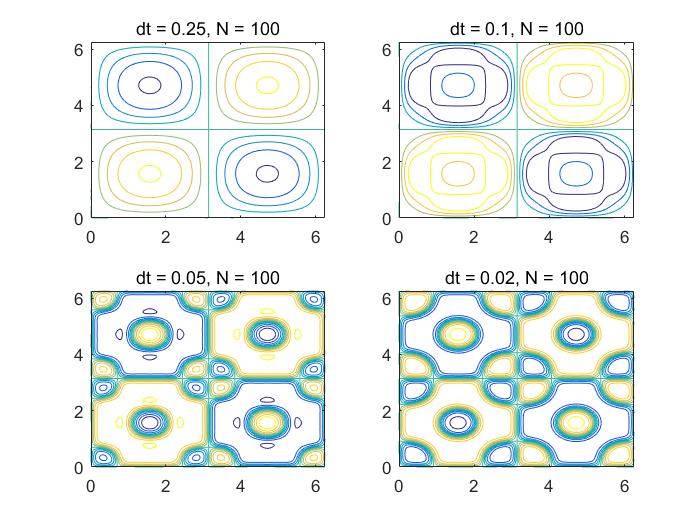
\includegraphics[scale=0.4]{Cahn_Hilliard_dt.png}
    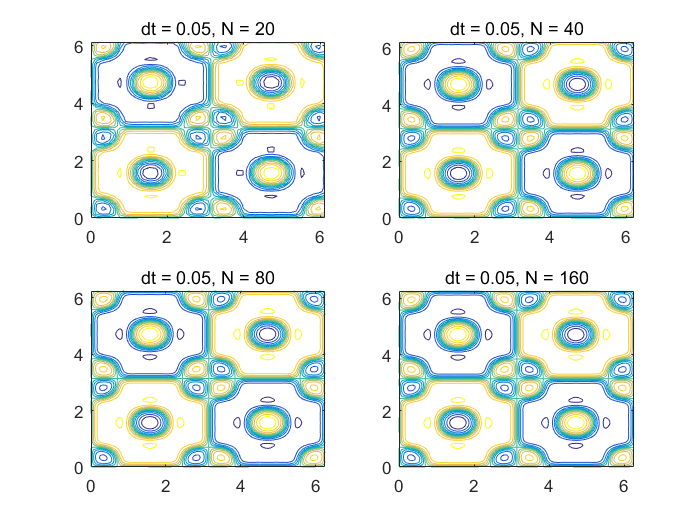
\includegraphics[scale=0.4]{Cahn_Hilliard_N.png}
    \caption{The numerical solutions of Cahn-Hailliard equation when time step $dt$ and nodes $N$ changs.}
    \label{im::2D_Cahn_Hilliard_parameter}
\end{figure}
In Figure \ref{im::2D_Cahn_Hilliard_parameter}, we choose the soltion when $T=2$ and the initial function 
\begin{equation}
    u_0(x,y)=sinxsiny
\end{equation}
We observe the difference between different $dt$ and $N$. Find that when $dt$ is not small enough, the Fourier Galerkin does not converges. And with $N$ growing, the solution can be more exactly but can not influence the convergence. 
\newpage
\section{Matlab Code}
\begin{lstlisting}
%Allen-Cahn equation
%parameter initialization
%2N + 1 is the number of the points, [a,b] is the domain, dt is the time step, eps is the parameter, u0=u(x,0)
%t is the beginning time, T is the ending time
N = 20;
a = 0; b = 2 * pi ; dt = 0.001; h = (b - a) / (2 * N + 1);
x = h * (0 : 2 * N)'; y = h * (0 : 2 * N)';
eps = 0.01; u0 = sin(x) * sin(y');
%u0 = 2 * rand(2 * N + 1) - 1;
t = 0; T = 1;

%initialization
%w is the nonlinear term, hatu is the spectral of u, A is the iteration matrix
%W1,W2 is the translation matrix for fft
wp = u0 - u0.^3;
hatup = spectral_fft2(u0);
j = -N : N;
j = j .^ 2;
A = zeros(2 * N + 1, 2 * N + 1);
for k = 1 : 2 * N + 1
    A(1 : 2 * N + 1, k) = 1 ./ (1 + dt * eps * (j(1 : 2 * N + 1) + j(k)));
end
up = u0;
j = 0 : 2 * N;
W1 = (exp(-2 * pi * N / (2 * N + 1) * j' * 1i) * exp(-2 * pi * N / (2 * N + 1) * j * 1i));
W2 = (exp(2 * pi * N / (2 * N + 1) * j' * 1i) * exp(2 * pi * N / (2 * N + 1) * j * 1i));

%Iteration, *p shows the value of time t, *n shows the value of time t+dt
while t < T 
    %calculate the spectral of w
    hatwp = ifft2(wp .* W1);
    
    %update the spectral of u
    hatun = (hatup  + dt .* hatwp ).*A;
    
    %transform the spectral to physical space, update u and w
    un = real(fft2(hatup) .* W2);
    wn = un - un.^3;
    
    %record residual
    res = max(abs(un - up));
    
    %time developing
    t = t + dt; up = un; wp = wn; hatup = hatun;
    
    %plot images
    %contour(X,Y,U);
    %pause(0.001);
end

%take in the end point
X=[x;b];
Y=[y;b];
U=[up up(1:2*N+1,1);up(1,1:2*N+1) up(1,1)];

%plot contour line
contour(X,Y,U);
        
\end{lstlisting}
\end{document}